\textbf{COLUNI 2021 -- Questão 31}\par\medskip Observe o mapa do Brasil abaixo.

\par

\textbf{Pontos extremos e fronteiras}

\par

% COLUNI-AUTO-FIGURES-BEGIN
\begin{figure}[htbp]
\centering
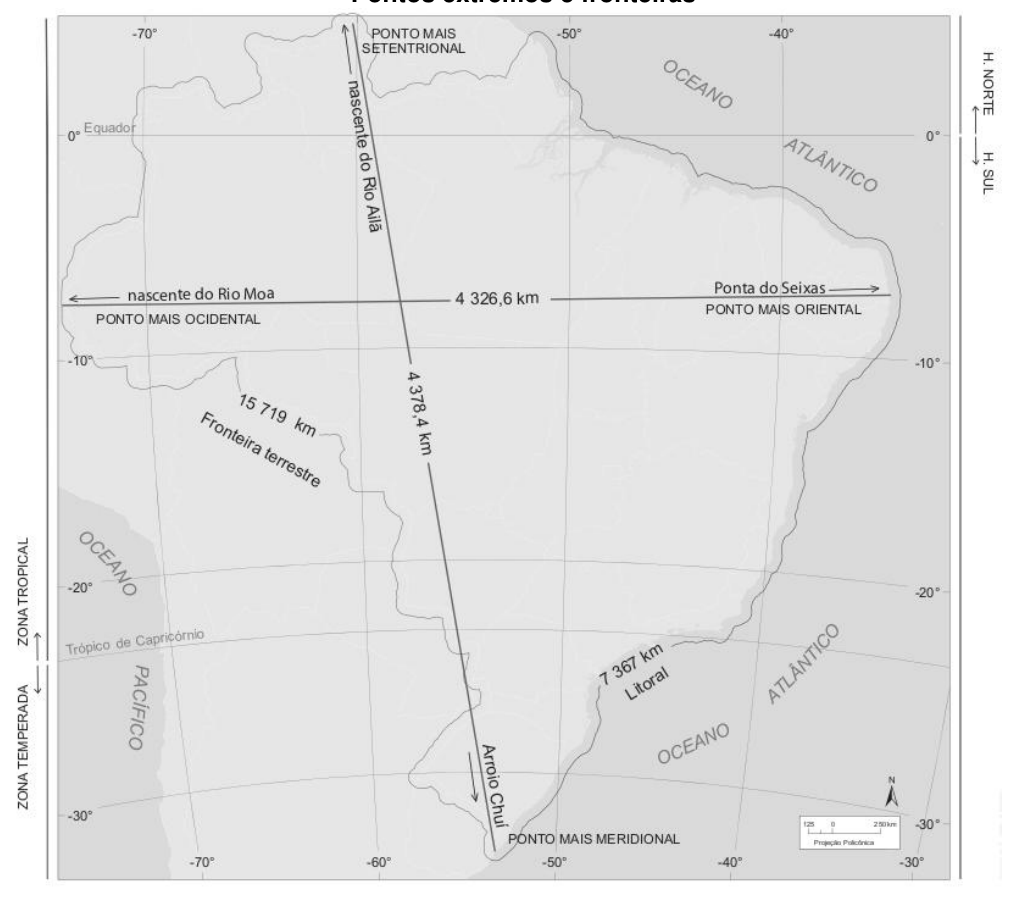
\includegraphics[width=0.95\linewidth]{static/simulados/coluni/figuras/2021/questao-31/figura-1.png}
\end{figure}
% COLUNI-AUTO-FIGURES-END

Disponível em: https://atlasescolar.ibge.gov.br/images/atlas/mapas\_brasil/brasil\_pontos\_extremos\_e\_fronteiras.pdf. Acesso em: 22 nov. 2020.

\par

Considerando a interpretação do mapa e os conhecimentos geográficos necessários, assinale a alternativa INCORRETA:

\begin{enumerate}
\item Os pontos extremos do norte e do sul do Brasil adotam o mesmo fuso horário.
\item A maior parte do território brasileiro está localizada no hemisfério sul e na zona tropical.
\item O Brasil é um país de grande extensão, cortado pelas linhas do Equador e do Trópico de Capricórnio.
\item A escala desse mapa não permite representação detalhada das áreas.\end{enumerate}
